\documentclass[12pt,twoside]{article}

%Packages
\usepackage[utf8]{inputenc}
\usepackage{amssymb}
\usepackage{amsmath}

\usepackage{enumerate}
\usepackage{tabularx,booktabs,mathrsfs,setspace}%
\usepackage{mathtools}
\usepackage{enumerate}
\usepackage{graphicx}
\usepackage{caption}
\usepackage[a4paper,top=20mm,bottom=20mm,left=20mm,right=20mm]{geometry}
\usepackage{appendix} % Add this line to define the "appendices" environment
\usepackage{hyperref} % Add this line for the \url command
\hypersetup{
	colorlinks=true,       % false: boxed links; true: colored links
	linkcolor=black,        % color of internal links,
	citecolor=black,
}

% Algorithm
\usepackage{algorithm}
\usepackage{algorithmic}

% For longtable
\usepackage{longtable}
\usepackage{booktabs}
\renewcommand{\arraystretch}{1.1}
\setlength{\tabcolsep}{3pt}


% ++++++++++++++++++++++++++Code global config begin++++++++++++++++++++++++++
% Code block universal settings, all lstdefinestyle must appeared below this block!
\usepackage{listings}
% use txtt global font
\usepackage[T1]{fontenc} % Add font options
\DeclareFixedFont{\codefont}{T1}{txtt}{m}{n}{12} % other options: txtt -> cmtt, pcr, fvm, zi4; m -> bx, n; 12 -> (fontsize)

% Define colors
\usepackage{color}
\usepackage{tikz} % colorlet need this
\definecolor{commentgreen}{rgb}{0,0.5,0}
\colorlet{framegray}{black!40}
\definecolor{stringred}{rgb}{0.6,0,0}

% Global config
\lstset{
    backgroundcolor=\color{gray!7},
    numbers = left, % show line number on the left
    numberstyle = \small\color{framegray}, % line number color
    basicstyle = \codefont, % code font
    columns = flexible, % make the spacing between characters compact
    keepspaces = true,  % keeps spaces in text, useful for keeping indentation of code (needs columns=flexible)
    % captionpos = b, % caption at the bottom
    commentstyle = \color{commentgreen}, % comment color
    frame = single, % display frame
    stringstyle = \color{stringred}, % Strings in red
    rulecolor = \color{framegray}, % frame color
    showstringspaces = false, % don't mark spaces in strings
    breaklines = true, % break long lines
    tabsize = 4, % tab size
}
% +++++++++++++++++++++++++++Code global config end+++++++++++++++++++++++++++

% ++++++++++++++++++++++++++Bash local config begin++++++++++++++++++++++++++
% Must placed below the global settings
% this will override the global settings
\lstdefinestyle{custombash}{
    language = bash,
    basicstyle = \ttfamily, % Monospaced font
    keywordstyle = \color{blue}\bfseries, % Keywords in bold blue
    stringstyle = \color{green}, % Strings in green
    commentstyle = \color{gray}, % Comments in gray
    morekeywords = {sudo, ls, cd, rm, mkdir}, % Add common Bash commands
}
% +++++++++++++++++++++++++++Bash local config end+++++++++++++++++++++++++++

% ++++++++++++++++++++++++++Python local config begin++++++++++++++++++++++++++
% Must placed below the global settings
% Custom colors for python only
\definecolor{emphblue}{rgb}{0,0,0.5}
\definecolor{keywordpink}{RGB}{128, 0, 128}
% this will override the global settings
\lstdefinestyle{custompython}{
    language = Python,
    emph = {__init__}, % Custom highlighting
    emphstyle = \color{emphblue},  % Highlighted words in deepblue
    keywordstyle = \color{keywordpink},
    upquote = true, % single quotes in straight quote
}
% ++++++++++++++++++++++++++++Python local config end++++++++++++++++++++++++++++

% ++++++++++++++++++++++++++MATLAB local config begin++++++++++++++++++++++++++
% Must placed below the global settings
% font and keyword need matlab-prettifier package
\usepackage[numbered,framed]{matlab-prettifier}
% this will override the global settings
\lstdefinestyle{custommatlab}{
    language = Matlab,
    style = Matlab-editor,
    basicstyle = \mlttfamily, % This font looks nice
    mlshowsectionrules = true, % show a line when encounter '%%'
    emph = {on, off}, % Custom highlighting
    emphstyle = \color{stringred},  % Highlighted words in stringred
    rulecolor = \color{framegray}, % reclaim frame color (because 'style = Matlab-editor' will overwrite the frame color defined in lstset)
}
% +++++++++++++++++++++++++++MATLAB local config end+++++++++++++++++++++++++++


\begin{document}

\begin{center}
    \textbf{ } \\
    \vspace{14em}
    {\huge \textsf{Source coding for \textit{the Game of Thrones}}} \\
    \vspace{1.5em}
    {\large \textsf{Second-order Markov Adaptive Approximation, Huffman and Fano Coding}} \\
    \vspace{1em}
    \vspace{1.5cm}
    \textbf{Name:} Jinming Ren, Yuhao Liu \\
    \vspace{0.5em}
    \textbf{UESTC ID:} 2022190908020, 2022190908022 \\
    % \textbf{UESTC ID:} ---, --- \\
    \vspace{0.5em}
    \textbf{UofG ID:} 2840216R, 2840218L \\
    % \textbf{UofG ID:} ---, --- \\
    \vspace{0.5em}
    \textbf{Date:} November 28, 2024 \\
    \vspace{0.5em}
    \vspace{1cm}
    \textbf{University:} UoG-UESTC Joint School \\
    \vspace{0.5em}
    \textbf{Location:} No.6 Research Build A240 \\
    % \textbf{Location:} --- \\
    \vspace{2cm}
\end{center}

\newpage
\tableofcontents

\newpage
\listoffigures
\listoftables
\newpage

\begin{abstract}
    In this article, we successfully implemented huffman and Fano coding to encode/denode the first three chapters of \textit{the Game of Thrones} and evaluated their raw performance in terms of the average code length, code rate, efficiency, and compression ratio in MATLAB. We also presented a new lossless coding scheme called 2nd-order Adaptive Markov Encoding (2nd-ord AME, abbreviated AME) coding and evaluated the overall performance when combined with huffman coding and fano coding.
\end{abstract}

\section{Introduction}

Source coding, a fundamental technique in data compression, plays a vital role in modern information transmission and storage. Its primary objective is to reduce the number of bits required to represent symbols from a source by leveraging their inherent statistical properties. This efficiency enables effective data storage and transmission while maintaining the integrity of the original information.

In this project, we explore the application of Huffman Coding and Fano Coding, two widely recognized entropy-based compression techniques. Huffman Coding, a lossless algorithm, is designed to assign shorter codes to frequently occurring symbols, making it highly efficient for sources with uneven symbol distributions. On the other hand, Fano Coding, while similar in principle, uses a different approach to partition symbols based on frequency.

Using MATLAB, we implemented both methods to encode and decode the first three chapters of a selected text, generating metrics such as average code length, code rate, efficiency, and compression ratio for comparison. Additionally, we introduced a important change-of-perspective that compression is essentially the same as prediction. Based on this idea, we introduced a novel pre-processing technique, Second-order Adaptive Markov Encoding (AME), designed to enhance the compression performance by uncovering structural patterns in the source text. The efficiency of AME was also evaluated.


\section{The Idea of AME Coding}

\subsection{Compression is Equivalent to Prediction}

In this section, we state the motivation and basic idea behind AME coding. 

Both huffman coding and fano coding are based on the assumption that the source is \textit{memoryless}. They are trying to approach the compression limit (which is the entropy of the source \cite{ref1}) given that the original source looks random. So they are called ``entropy coding''. However, in practice, the texts inherently take some structures that cannot be explicitly captured by any relative simple models. These structures are not considered when performing entropy coding, so we wasted some potential compression ratio.

No matter what coding method we choose, such as LZ77 \cite{ref6, ref7}, the last step of them is always entropy coding. But entropy coding is well-understood and mature (Huffman being the ``optimal'' in some sense). Therefore, the only way to improve compression ratio is to uncover the structure of the source. We need to design a better model first to capture and hiding those structures while exposing the true ``memoryless components'' of the source, then the utility of entropy coding can be maximized.

The basic idea behind AME coding is that \textit{compression} is equivalent to \textit{prediction}. We are essentially building a same text predictor in both sides of the transmitter and the receiver. As long as the predicted next character matches the true one, that character is not considered as the ``memoryless component'' of the source (it depends on the history text). But if the predicted one doesn't match the true one, this means there are somewhat ``random'' factors come into play. If we can proposed some encoding strategy that makes the predictor works exactly the same on both the transmitter and receiver, we only need to transmit the ``memoryless components'' and the number of correct predictions. 

For example, if we want to extract the ``memoryless components'' of the following content:

% literal bash commands
\begin{lstlisting}[language=bash, style=custombash]
Information theory is interesting.
\end{lstlisting}

Feed it into the predictor, suppose we can correctly predict the character in position 2, 5-11, 15-19, 21-22, 26-34, we only need to transmit the initial letter that cannot be predicted together with the number of correct predictions:

\begin{lstlisting}[language=bash, style=custombash]
I1fo7 th5i2int9
\end{lstlisting}

The rest letters are somehow losed some internal dependence and can be approximately considered as ``memoryless''. 

We can see in this example the efficiency of compression directly relies on how well we extract the ``memoryless components'' of the text, in other words, the performance of the predictor. Since human language is the product of human mind, which definitely cannot be modelled using just a few parameters. An accurate predictor would need millions of parameters, which is essentially a neural network \cite{ref5}. However, due to time and space complexity, using a neural network to predict the next character is not feasible in practice. However, we can use a simpler model called markov chain to capture some of the structures in the text. The markov chain is built with the encoding/decoding process, so it is called ``adaptive''.

\subsection{Mechanism of AME Coding}
\label{sec:markov}


We assume no prior knowledge of the source. So the predictor is built simultaneously with the encode/decode process. We used markov chain to model the process. With the inspiration in \cite{ref1}, we use a tree (a weighted digraph in formal terms) to represent the markov process. The algorithm for AME encoding and decoding are shown in Algorithm~\ref{alg:markov_encode} and \ref{alg:markov_decode} in Appendix~\ref{app:AMEalgo1} and \ref{app:AMEalgo2}. The codes are written in Python and can be found in the appendix~\ref{app:markov_encode} and \ref{app:markov_decode}.

\begin{figure}[h!]
    \centering
    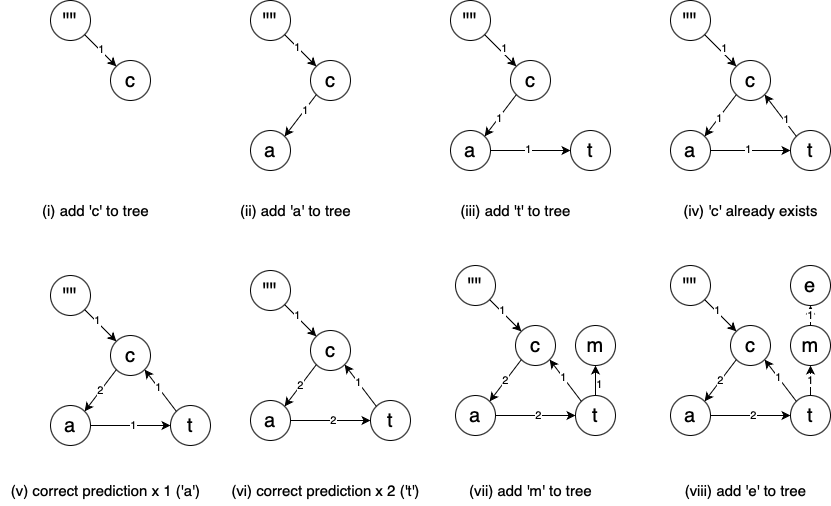
\includegraphics[width=\textwidth]{AMEtree.png}
    \caption{The AME tree construction precedure}
    \label{fig:AMEtree}
\end{figure}

We will take an example to show how AME works. Let's consider the following text:

\begin{lstlisting}[language=bash, style=custombash]
catcatme
\end{lstlisting}

The building process is shown in Figure~\ref{fig:AMEtree}. It is summarized as follows:

\begin{enumerate}
    \item Initially, the tree is empty. The first character in the text is \texttt{`c'}, so we add \texttt{`c'} to the AME tree, mark the weight 1 (since first appearance) and add it directly to the output buffer. 
    \item The next character is \texttt{`a'}, so we add \texttt{`a'} to the AME tree, mark the weight also 1 and also add it to the output buffer. 
    \item Repeat this process until we could possibly ``predict'' the next character, i.e., the arrow with the highest weight in the tree from the current character leads to the correct character appeared in the text (If there are multiple arrows with the same highest weight, we take the most recent one).
    \item The first correct prediction is the 5th character (\texttt{`a'}). We increase the weight from \texttt{`c'} to \texttt{`a'} by 1 and continue to predict the next character.
    \item The next prediction (\texttt{`t'}) is also right. We increase the weight from \texttt{`a'} to \texttt{`t'} by 1 and continue to predict the next character.
    \item But the next two characters after \texttt{`t'} are \texttt{`m'} and \texttt{`e'}, which are not even in the tree! Thus we first add the number of correct predictions in history (which is 2) and then add the two new characters (\texttt{`m'} and \texttt{`e'}) to the tree. 
\end{enumerate}

Therefore, the output buffer is:

\begin{lstlisting}[language=bash, style=custombash]
catc2me
\end{lstlisting}

It saves one character in this case, but it can be more significant in a larger text. Part of the AME-encoded \texttt{original.txt} in shown in Appendix~\ref{lst:processedpart}.


\section{Entropy Coding Review}
\subsection{Mechanism of Huffman coding}
\label{sec:huffman}

Huffman coding is a lossless data compression algorithm proposed by David A. Huffman in 1952 \cite{ref1}. It reduces the size of data by assigning variable-length codes to characters based on their frequencies of occurrence \cite{ref2, ref3}. The core principle behind Huffman coding is to assign shorter codes to more frequent characters and longer codes to less frequent ones. The process begins with the construction of a frequency table, which lists each character and its corresponding frequency in the data. From there, a binary tree is built by repeatedly combining the two nodes with the lowest frequencies into a new node. This is the clever part, it builds from the ground up (instead of from the node to the leaves). This process continues until all nodes are merged into a single tree, with the root node representing the entire data set. The structure of this tree enables the generation of optimal, prefix-free binary codes, where each character's code is determined by its position in the tree. In the final step, the original characters in the data are replaced with their corresponding Huffman codes, achieving the desired compression. We perform this process in MATLAB and we visualize the tree in the figure in Appendix~\ref{app:huffmanTree}.

\subsection{Mechanism of Fano coding}
\label{sec:fano}

Fano coding is another lossless data compression algorithm that assigns variable-length codes to characters based on their frequencies, similar to Huffman coding. The key principle behind Fano coding is to recursively divide the data set into two parts, ensuring that the frequencies of the characters in each part are as balanced as possible, and then assign binary codes accordingly. The process begins with constructing a frequency table, listing each character alongside its frequency. The next step is to split the set of characters into two subsets, aiming to balance the total frequencies of both subsets. Each subset is then assigned a binary digit (0 or 1), and the process is repeated for each subset. As the binary tree is built, characters are assigned codes based on the path from the root to the leaf node representing that character. Finally, the original characters in the data are replaced by their corresponding Fano codes, resulting in compression. Like Huffman coding, Fano coding ensures that the encoded data is more compact without any loss of information. However, its encoding efficiency is quite low when dealing with source symbols that have relatively uniformly distributed probabilities.

All MATLAB codes of the encode/decode process of Huffman and Fano coding can be found in the appendix~\ref{app:huffman} and \ref{app:fano}.

\section{Implementation}

We performed two seperated experiments for different purposes. The first is to realize Huffman and Fano coding on the original text and perform evaluations. Given that Huffman coding is the optimal method for generating codes, especially when there are significant differences in the probabilities of occurrence for different source symbols, it should significantly outperform the Fano coding technique in terms of coding effectiveness \cite{ref3, ref4}. The second is to combine AME coding with Huffman and Fano coding and evaluate the performance of the new scheme.

\subsection{Without AME}

The encode/decode process is shown in the form of a flowchart shown in Figure~\ref{fig:without-ame}.

\begin{figure}[h!]
    \centering
    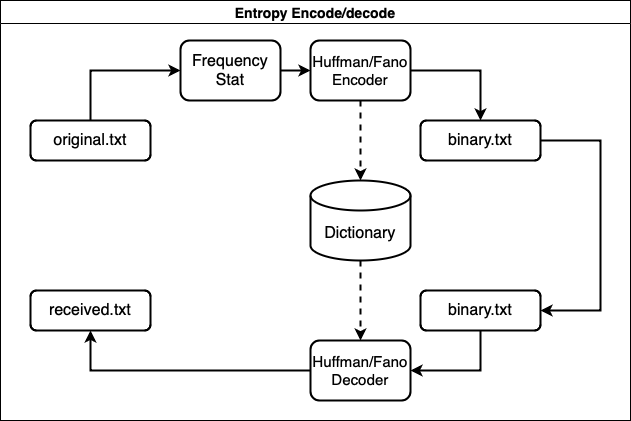
\includegraphics[width=0.7\textwidth]{without-ame.png}
    \caption{Flowchart of the experiment without AME}
    \label{fig:without-ame}
\end{figure}

The content in \texttt{original.txt} contains the first three chapters of \textit{the Game of Thrones}. Part of the \texttt{original.txt} is shown in Appendix~\ref{lst:originalpart}.

In order to perform huffman/fano coding on the text, we first need to calculate the frequency of each character in the text. According to statistics, the distribution of all characters in shown in Figure~\ref{fig:originalStat}. The detailed frequency table of each character is shown in Appendix~\ref{app:originalStat}.

\begin{figure}[h!]
    \centering
    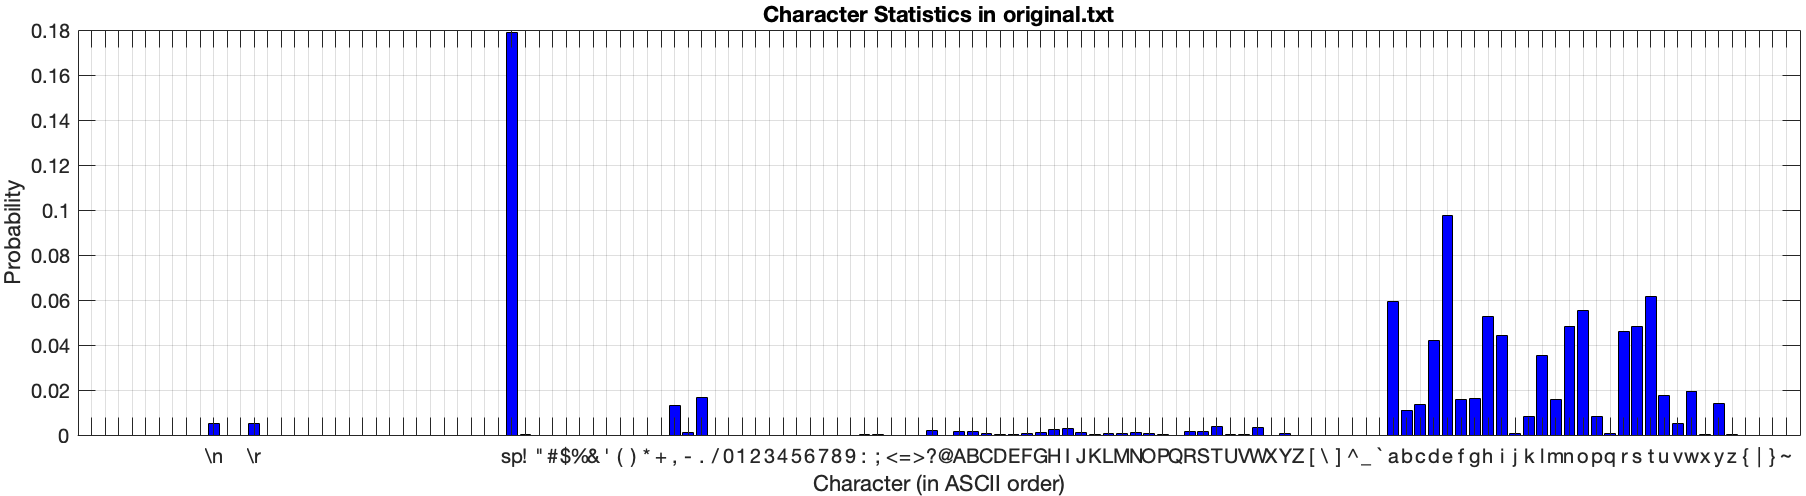
\includegraphics[width=\textwidth]{originalStat.png}
    \caption{Distribution of each character in the \texttt{original.txt}}
    \label{fig:originalStat}
\end{figure}

According to the frequency of each character, we can create the Huffman/fano tree based on the methods in Section~\ref{sec:huffman} and \ref{sec:fano} and generate the huffman/fano dictionaries\footnote{The dictionaries together with all codes can be found on \url{https://github.com/Marcobisky/ame-entropy-source-coding}}. We then use this dictionary to encode the text and calculate the four main metrics including average code length $\bar{L}$, code rate $R$, efficiency $\eta$, and compression ratio $\xi$. The results are shown in Section~{sec:result}. 

Then we constructed the encoded text in binary form (\texttt{binary.txt}). Part of the content of (\texttt{binary\_huffman.txt}) is shown in Appendix~\ref{lst:binaryhuffmanpart}. Then we send the encoded text (\texttt{binary.txt}) to the receiver and decode it using the same dictionary to recover the original text.



\subsection{With AME}

The experiment procedure of the encode/decode process in shown in Figure~\ref{fig:with-ame}.

\begin{figure}[h!]
    \centering
    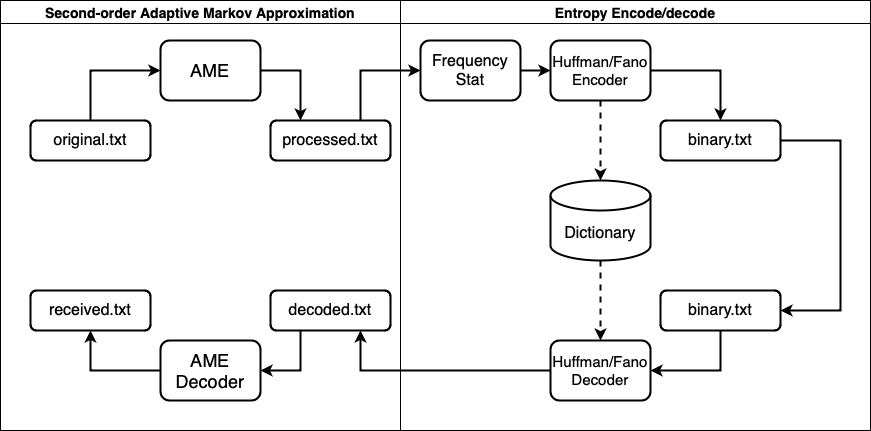
\includegraphics[width=0.9\textwidth]{with-ame2.png}
    \caption{Flowchart of the experiment with AME}
    \label{fig:with-ame}
\end{figure}

The only difference of this part is that we added a block called ``Second-order Adaptive Markov Approximation'' before applying the entropy encode/decode. Using the method in Section~\ref{sec:markov}, we get the AME-encoded text (\texttt{processed.txt}). Part of the content of (\texttt{processed.txt}) is shown in Appendix~\ref{lst:processedpart}.

Then we apply the same procedure for \texttt{processed.txt} as we did for \texttt{original.txt}. Note this time the frequency of each character is different from the original text. For example, there are no numbers in \texttt{original.txt} but there are in \texttt{processed.txt}. According to statistics, the distribution of all characters in shown in Figure~\ref{fig:processedStat}. The detailed frequency table of each character is shown in Appendix~\ref{app:processedStat}.

\begin{figure}[h!]
    \centering
    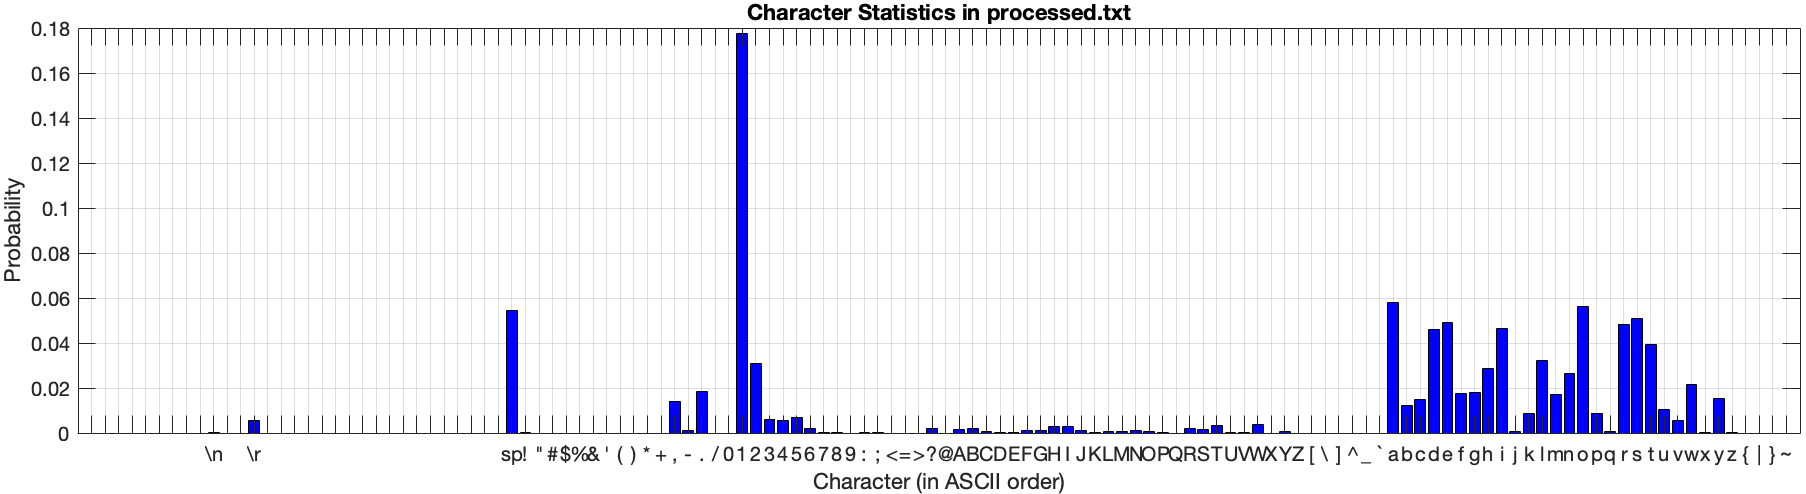
\includegraphics[width=\textwidth]{processedStat.png}
    \caption{Distribution of each character in the \texttt{processed.txt}}
    \label{fig:processedStat}
\end{figure}






After encoded into binary form, we send it to the receiver and decode it using the same dictionary to get the \texttt{decoded.txt}. However this is not the final result, we need to use the AME decoder to recover the original text. The AME decoder decodes the \texttt{decoded.txt} with no prior knowledge of the source. Since the markov chain is constructed in the same way, we are guaranteed to get the original text back.


\section{Results and Discussion}
\label{sec:result}

\subsection{Performance comparison between Huffman and Fano coding}

The four main metrics of Huffman and Fano coding are shown in Table~\ref{tab:metrics}.

\begin{table}[h!]
    \caption{Performance Metrics for Huffman and Fano Coding}
    \label{tab:metrics}
    \centering
    \begin{tabular}{l|ccc}
    \toprule
    \textbf{Parameter} & \textbf{Symbol} & \textbf{Huffman} & \textbf{Fano} \\ \hline
    Average Code Length & $\bar{L}$ & 4.5023 & 8.4244 \\ 
    Code Rate & $R$ & 0.9909 & 0.5282      \\ 
    Efficiency & $\eta$ & 0.9909 & 0.5282  \\ 
    Compression Rate & $\xi$ & 0.5628 & 1.0530  \\ 
    \bottomrule
    \end{tabular}
\end{table}

The four metrics are defined in Appendix~\ref{app:metrics}. Table~\ref{tab:metrics} shown that Huffman coding outperforms Fano coding in all four metrics, which matches the fact that Huffman coding is the ``optimal'' coding strategy in the usual sense.

However, we noticed that the compression ratio achieved by Fano coding is greater than 1, which is unreasonable. With the following analysis, we claim it's because this text is \textit{unsuitable} for Fano Coding. Compared to other coding methods, the effectiveness of Fano Coding relies heavily on the uneven frequency distribution of symbols. Specifically, Fano Coding performs best when certain symbols appear very frequently while others are relatively rare. This frequency disparity allows shorter codes to be assigned to frequently occurring symbols, enabling compression.

However, in this text, the symbol frequency distribution is relatively uniform. The probability difference between frequently occurring symbols (such as spaces and letters) and rare symbols (such as punctuation marks) is not significant. In such cases of uniform symbol distribution, Fano Coding may fail to significantly reduce the file size. In fact, due to redundancy and long codewords, it may even increase the file size, leading to a compression ratio greater than 1. Moreover, we calculated the variance of the symbol frequencies in this text as follows:

% literal matlab code
\begin{lstlisting}[language=Matlab, style=custommatlab]
>> var(probabilities)
ans = 
    8.9864e-04
\end{lstlisting}

It is evident that the variance of the frequencies corresponding to these characters is very small, which further validates the point that the frequency distribution of symbols in this text is relatively uniform.

All above further highlights the superiority of Huffman Coding.

\subsection{Performance analysis of AME coding}

Since we pre-processed the \texttt{original.txt} before fed into the entropy coding, we cannot directly compute the four metrics of it. So we compared the length of \texttt{binary.txt} file generated in the two methods. 

Let the length of the \texttt{binary\_huffman.txt} and \texttt{binary\_fano.txt} be $L_{\text{h}}$ and $L_{\text{f}}$, respectively. Table~\ref{tab:amematrics} shows how using AME could save the length of the binary file.

% \begin{table}[h!]
%     \caption{AME saves the length of binary file}
%     \label{tab:amematrics}
%     \centering
%     \begin{tabular}{l||cc}
%     \toprule
%      & $L_{\text{h}}$ & $L_{\text{f}}$ \\ \hline
%     With AME & 207797 & 209343  \\ 
%     Without AME & 217014 & 218913 \\ 
%     Saved & 5.25\% & 4.37\% \\ 
%     \bottomrule
%     \end{tabular}
% \end{table}

\begin{table}[h!]
    \caption{AME shortened the length of the binary file}
    \label{tab:amematrics}
    \centering
    \begin{tabular}{l|cccc}
    \toprule
    \textbf{Parameter} & \textbf{Symbol} & \textbf{With AME} & \textbf{Without AME} & \textbf{Improved} \\ \hline
    Huffman Binary Length & $L_{\text{h}}$ & 207797 & 217014 & 5.25\%  \\ 
    Fano Binary Length & $L_{\text{f}}$ & 209343 & 218913 & 4.37\% \\ 
    \bottomrule
    \end{tabular}
\end{table}

This result shown that AME + Huffman/Fano coding could save about 5.25\% and 4.37\% of the length of the binary file, respectively. 


\section{Conclusion and Future Work}

In this project, we successfully implemented the Huffman Coding technique using MATLAB, creating compressed files optimized for transmission and storage. Additionally, by comparing the results with Fano Coding, we explored the efficiency and optimization of Huffman Coding.

Furthermore, we introduced a new lossless coding scheme called 2nd-order Adaptive Markov Encoding (AME) coding, which serves as a pre-processor before applying entropy coding. It aims to uncover the structure of the source text and improve the compression ratio by extracting the ``memoryless components'' of the text. 

Future work could involve using higher order Markov models or new mathematical models to capture more complex structures in the text, potentially furthermore improving the compression ratio. 



\addcontentsline{toc}{section}{References}
\begin{thebibliography}{9}
    \bibitem{ref1} C. E. Shannon, ``A Mathematical Theory of Communication,'' \textit{The Bell System Technical Journal}, vol. 27, no. 3, pp. 379–423, July 1948, doi: 10.1002/j.1538-7305.1948.tb01338.x.

    \bibitem{ref6} J. Ziv and A. Lempel, “A universal algorithm for sequential data compression,” \textit{IEEE Trans}. Inform. Theory, vol. 23, no. 3, pp. 337–343, May 1977, doi: 10.1109/TIT.1977.1055714.

    \bibitem{ref7} A. D. Wyner and J. Ziv, “The sliding-window Lempel-Ziv algorithm is asymptotically optimal,” \textit{Proc. IEEE}, vol. 82, no. 6, pp. 872–877, Jun. 1994, doi: 10.1109/5.286191.

    \bibitem{ref5} T. Sharma et al., ``A Survey on Machine Learning Techniques for Source Code Analysis,'' Sep. 13, 2022, arXiv: arXiv:2110.09610. doi: 10.48550/arXiv.2110.09610.

    \bibitem{ref2} Advances in Communication and Computing Technologies (ICACACT 2014), Mumbai, India, 2014, pp. 1-6, doi: 10.1109/EIC.2015.7230711.

    \bibitem{ref3} N. Dhawale, ``Implementation of Huffman algorithm and study for optimization,'' 2014 International Conference on Advances in Communication and Computing Technologies (ICACACT 2014), Mumbai, India, 2014, pp. 1-6, doi: 10.1109/EIC.2015.7230711.

    \bibitem{ref4} S. Congero and K. Zeger, ``Competitive Advantage of Huffman and Shannon-Fano Codes,'' in \textit{IEEE Transactions on Information Theory}, vol. 70, no. 11, pp. 7581-7598, Nov. 2024, doi: 10.1109/TIT.2024.3417010.




\end{thebibliography}

\newpage
\appendix

\begin{appendices}

\section{AME Coding Scheme}
\subsection{AME encode algorithm}
\label{app:AMEalgo1}

\begin{algorithm}
    \caption{Adaptive Markov Encoding}
    \label{alg:markov_encode}
    \begin{algorithmic}[1]
    \REQUIRE Input file \texttt{source.txt}, Output file \texttt{markov\_encoded.txt}
    \ENSURE Encoded text stored in \texttt{markov\_encoded.txt}
    \STATE Initialize an empty tree \texttt{tree}, list \texttt{encoded\_output}, and counter \texttt{correct\_predictions = 0}
    \STATE Read \texttt{source\_text} from \texttt{source.txt}
    \FOR{\texttt{i = 1} to \texttt{length(source\_text)}}
        \STATE \texttt{current\_char = source\_text[i]}
        \IF{\texttt{i == 1}} 
            \STATE Append \texttt{current\_char} to \texttt{encoded\_output}
            \STATE Add root-to-\texttt{current\_char} transition to \texttt{tree}
        \ELSE
            \STATE Predict next character using \texttt{tree}: \texttt{prediction = predict\_next(tree, prev\_char)}
            \IF{\texttt{prediction == current\_char}}
                \STATE Increment \texttt{correct\_predictions}
            \ELSE
                \IF{\texttt{correct\_predictions > 0}}
                    \STATE Append \texttt{correct\_predictions} to \texttt{encoded\_output}
                    \STATE Reset \texttt{correct\_predictions = 0}
                \ENDIF
                \STATE Append \texttt{current\_char} to \texttt{encoded\_output}
            \ENDIF
            \STATE Add transition \texttt{prev\_char $\to$ current\_char} to \texttt{tree}
        \ENDIF
        \STATE \texttt{prev\_char = current\_char}
    \ENDFOR
    \IF{\texttt{correct\_predictions > 0}}
        \STATE Append \texttt{correct\_predictions} to \texttt{encoded\_output}
    \ENDIF
    \STATE Write \texttt{encoded\_output} to \texttt{markov\_encoded.txt}
    \end{algorithmic}
\end{algorithm}
\newpage
\subsection{AME decode algorithm}
\label{app:AMEalgo2}

\begin{algorithm}
    \caption{Adaptive Markov Decoding}
    \label{alg:markov_decode}
    \begin{algorithmic}[1]
    \REQUIRE Input file \texttt{markov\_encoded.txt}, Output file \texttt{markov\_decoded.txt}
    \ENSURE Decoded text stored in \texttt{markov\_decoded.txt}
    \STATE Initialize an empty tree \texttt{tree}, list \texttt{decoded\_output}
    \STATE Read \texttt{encoded\_text} from \texttt{markov\_encoded.txt}
    \STATE \texttt{i = 1}
    \WHILE{\texttt{i $\leq$ length(encoded\_text)}}
        \STATE \texttt{current\_char = encoded\_text[i]}
        \IF{\texttt{i == 1}}
            \STATE Append \texttt{current\_char} to \texttt{decoded\_output}
            \STATE Add root-to-\texttt{current\_char} transition to \texttt{tree}
        \ELSE
            \STATE \texttt{prev\_char = decoded\_output[last]}
            \IF{\texttt{current\_char} is a digit}
                \STATE Extract full number as \texttt{repeat\_count}
                \STATE Predict next character using \texttt{tree}: \texttt{prediction = predict\_next(tree, prev\_char)}
                \FOR{\texttt{j = 1} to \texttt{repeat\_count}}
                    \STATE Append \texttt{prediction} to \texttt{decoded\_output}
                    \STATE Add transition \texttt{prev\_char $\to$ prediction} to \texttt{tree}
                    \STATE \texttt{prev\_char = prediction}
                \ENDFOR
            \ELSE
                \STATE Append \texttt{current\_char} to \texttt{decoded\_output}
                \STATE Add transition \texttt{prev\_char $\to$ current\_char} to \texttt{tree}
            \ENDIF
        \ENDIF
        \STATE \texttt{i = i + 1}
    \ENDWHILE
    \STATE Write \texttt{decoded\_output} to \texttt{markov\_decoded.txt}
    \end{algorithmic}
\end{algorithm}

\newpage
\subsection{Python code for AME encoding}
\label{app:markov_encode}

\lstinputlisting[caption={AME encoder}, label={lst:markov_encode}, language=Python, style=custompython]{../markovpy/adaptive_markov_encode.py} % python

\newpage
\subsection{Python code for AME decoding}
\label{app:markov_decode}

\lstinputlisting[caption={AME decoder}, label={lst:markov_decode}, language=Python, style=custompython]{../markovpy/adaptive_markov_decode.py} % python

\newpage
\section{Huffman Tree Visualization}
\subsection{Huffman Tree Generated for \texttt{original.txt}}
\label{app:huffmanTree}

\begin{figure}[h!]
    \centering
    \hspace*{-1.3cm}
    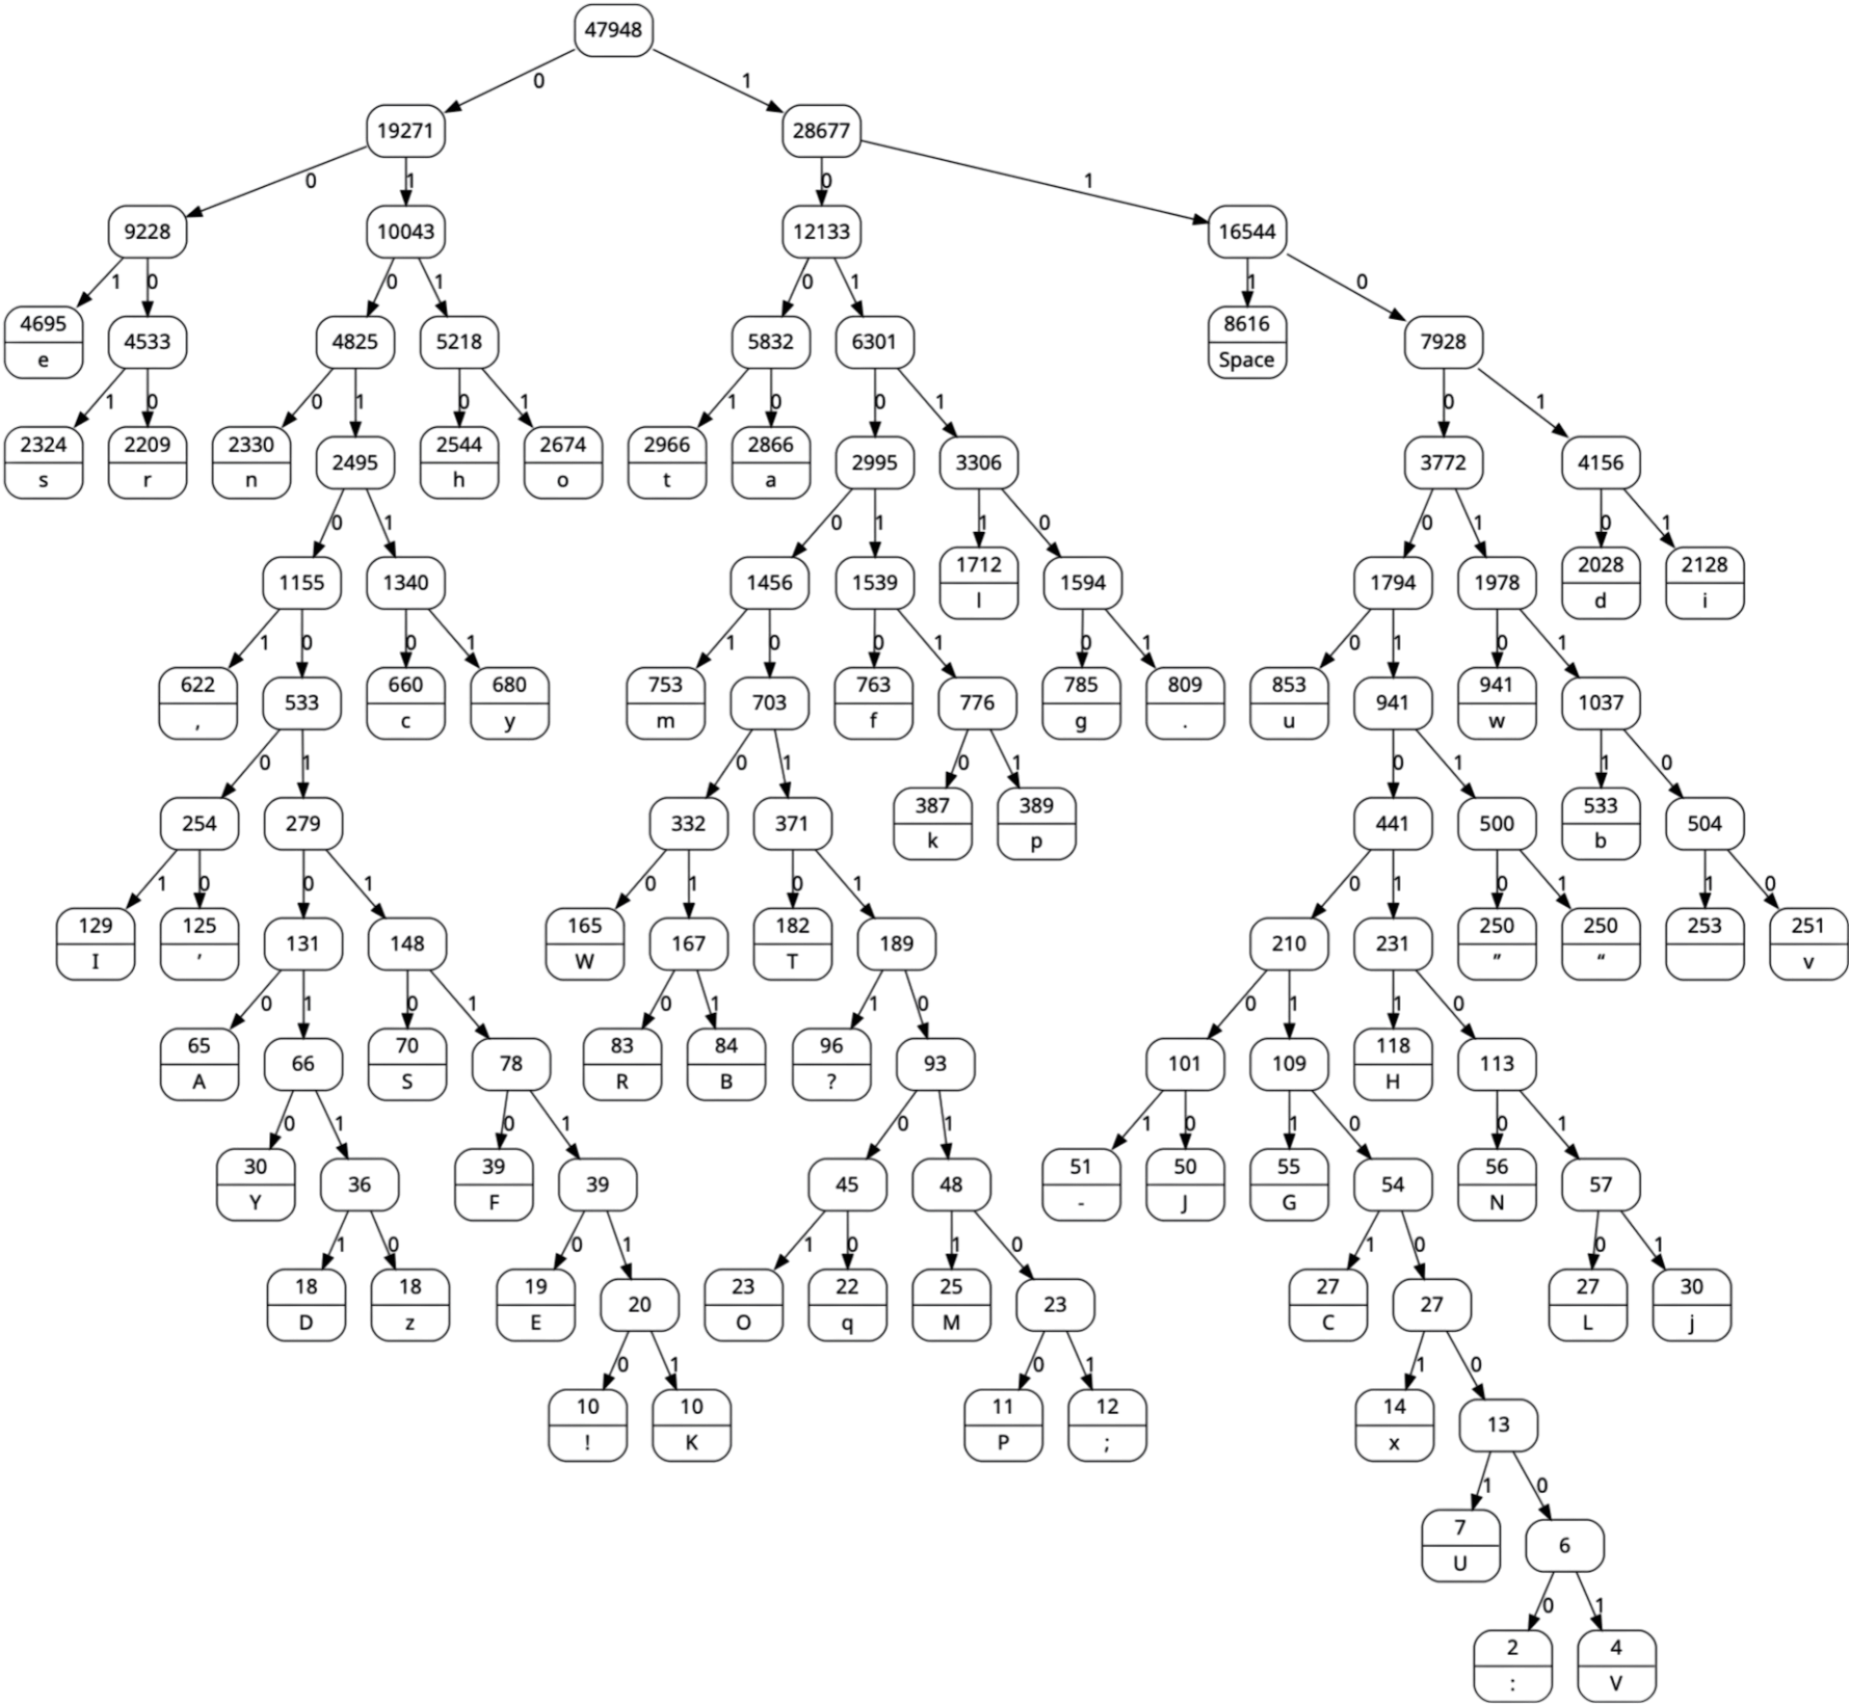
\includegraphics[width=1.15\textwidth]{huffmanTree.png}
    \caption{Huffman tree visualized for \texttt{original.txt}}
    \label{fig:huffmanTree}
\end{figure}

\newpage
\subsection{Fano Tree Generated for \texttt{processed.txt}}
\label{app:huffmanTreeAME}

\begin{figure}[h!]
    \centering
    \hspace*{-1.4cm}
    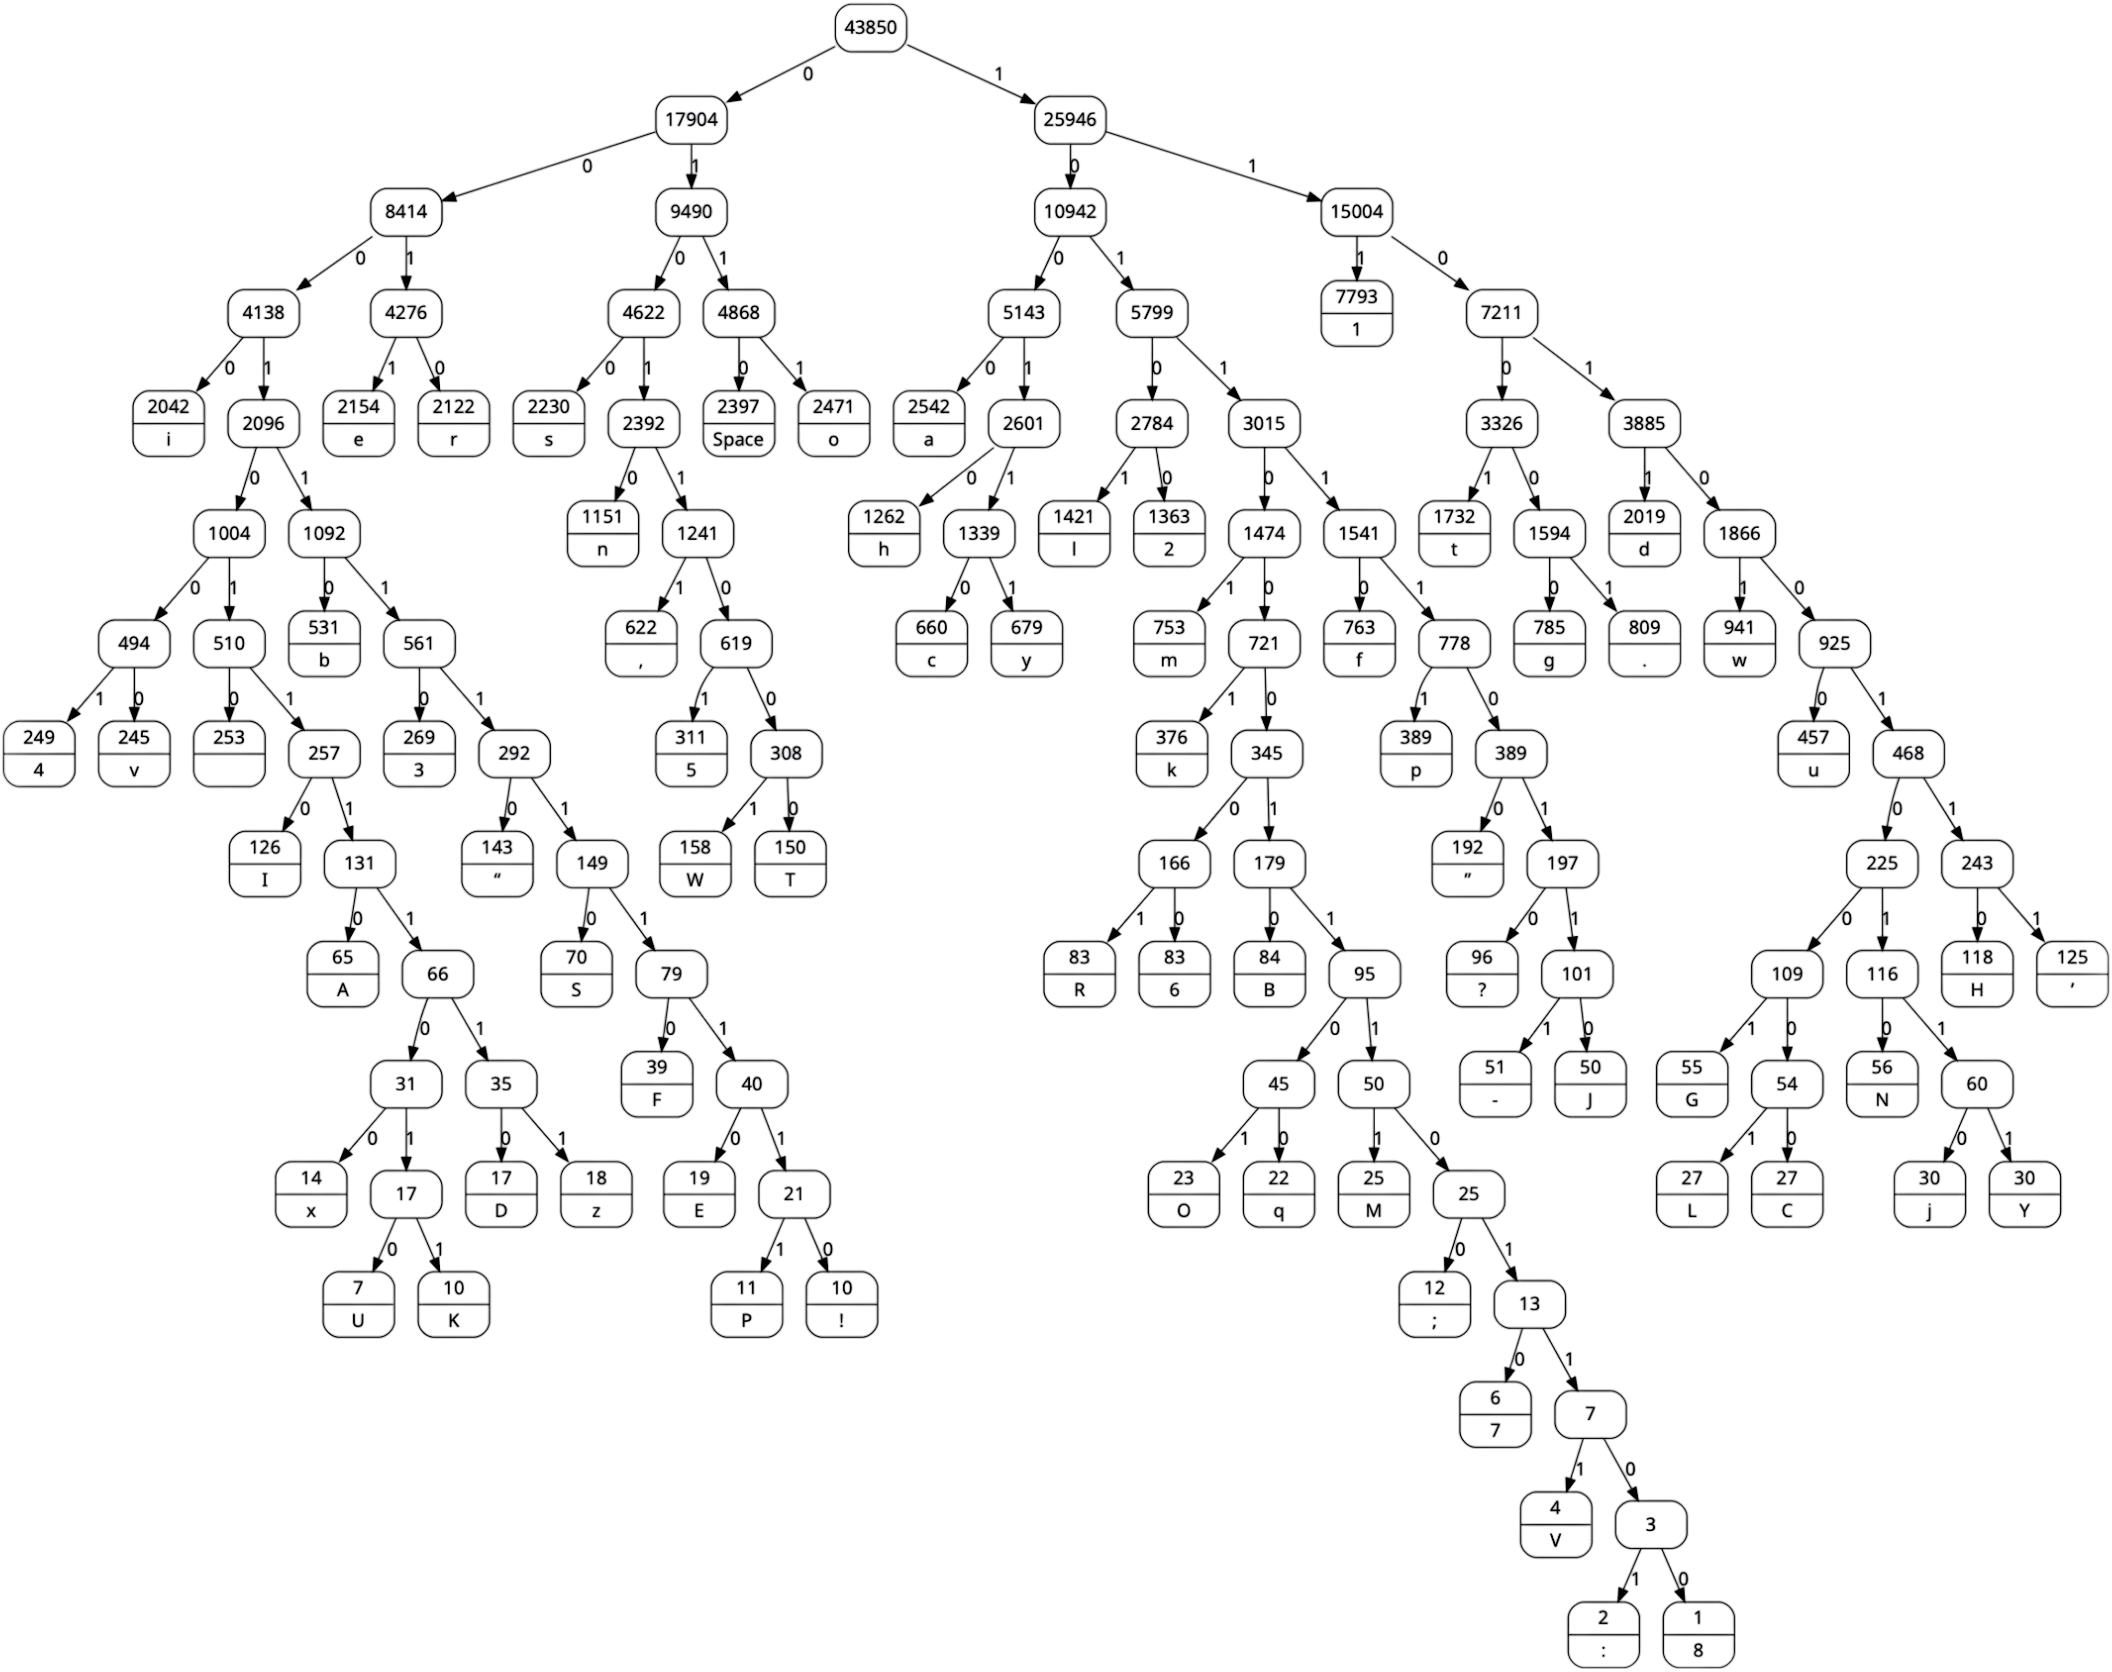
\includegraphics[width=1.15\textwidth]{huffmanTree_ame.png}
    \caption{Huffman tree visualized for \texttt{processed.txt}}
    \label{fig:huffmanTreeAME}
\end{figure}


\newpage
\section{Entropy Coding Scheme}
\subsection{MATLAB code for Huffman encode/decode procedure}
\label{app:huffman}

\lstinputlisting[caption={Huffman encode procedure (without AME example)}, language=Matlab, style=custommatlab]{../huffman/withoutAME/huffman_encode.m} % matlab code from file

\lstinputlisting[caption={Huffman decode procedure (without AME example)}, language=Matlab, style=custommatlab]{../huffman/withoutAME/huffman_decode.m} % matlab code from file

\lstinputlisting[caption={Main function to perform Huffman encode/decode}, language=Matlab, style=custommatlab]{../huffman/withoutAME/mainHuffman.m} % matlab code from file

\newpage
\subsection{MATLAB code for Fano encode/decode procedure}
\label{app:fano}

\lstinputlisting[caption={Fano encode procedure (without AME example)}, language=Matlab, style=custommatlab]{../fano/withoutAME/fano_encode.m} % matlab code from file

\lstinputlisting[caption={Fano decode procedure (without AME example)}, language=Matlab, style=custommatlab]{../fano/withoutAME/fano_decode.m} % matlab code from file

\lstinputlisting[caption={Main function to perform Fano encode/decode}, language=Matlab, style=custommatlab]{../fano/withoutAME/mainFano.m} % matlab code from file

\newpage
\section{Characters Statistics}
\subsection{Statistics in \texttt{original.txt}}
\label{app:originalStat}

\begin{longtable}{ccc||ccc||ccc}
    \caption{Frequency of each character in \texttt{original.txt}}
    \label{tab:originalStat} \\
    \toprule
    \textbf{ASCII} & \textbf{Char} & \textbf{Probability} & \textbf{ASCII} & \textbf{Char} & \textbf{Probability} & \textbf{ASCII} & \textbf{Char} & \textbf{Probability} \\ \hline
    \endfirsthead
    10 & \textbackslash n & 0.005249 & 32 & sp & 0.178751 & 65 & A & 0.001349 \\
    13 & \textbackslash r & 0.005249 & 33 & ! & 0.000207 & 66 & B & 0.001743 \\
    44 & , & 0.012904 & 45 & - & 0.001058 & 67 & C & 0.000560 \\
    46 & . & 0.016784 & 58 & : & 0.000041 & 68 & D & 0.000373 \\
    59 & ; & 0.000249 & 63 & ? & 0.001992 & 69 & E & 0.000394 \\
    70 & F & 0.000809 & 71 & G & 0.001141 & 72 & H & 0.002448 \\
    73 & I & 0.002676 & 74 & J & 0.001037 & 75 & K & 0.000207 \\
    76 & L & 0.000560 & 77 & M & 0.000519 & 78 & N & 0.001162 \\
    79 & O & 0.000477 & 80 & P & 0.000228 & 82 & R & 0.001722 \\
    83 & S & 0.001452 & 84 & T & 0.003776 & 85 & U & 0.000145 \\
    86 & V & 0.000083 & 87 & W & 0.003423 & 89 & Y & 0.000622 \\
    97 & a & 0.059459 & 98 & b & 0.011058 & 99 & c & 0.013693 \\
    100 & d & 0.042074 & 101 & e & 0.097405 & 102 & f & 0.015830 \\
    103 & g & 0.016286 & 104 & h & 0.052779 & 105 & i & 0.044148 \\
    106 & j & 0.000622 & 107 & k & 0.008029 & 108 & l & 0.035518 \\
    109 & m & 0.015622 & 110 & n & 0.048339 & 111 & o & 0.055476 \\
    112 & p & 0.008070 & 113 & q & 0.000456 & 114 & r & 0.045829 \\
    115 & s & 0.048215 & 116 & t & 0.061534 & 117 & u & 0.017697 \\
    118 & v & 0.005207 & 119 & w & 0.019522 & 120 & x & 0.000290 \\
    121 & y & 0.014108 & 122 & z & 0.000373 &  &  &  \\
    \bottomrule
\end{longtable}

\newpage
\subsection{Statistics in \texttt{processed.txt}}
\label{app:processedStat}

\begin{longtable}{ccc||ccc||ccc}
    \caption{Frequency of each character in \texttt{processed.txt}}
    \label{tab:processedStat} \\
    \toprule
    \textbf{ASCII} & \textbf{Char} & \textbf{Probability} & \textbf{ASCII} & \textbf{Char} & \textbf{Probability} & \textbf{ASCII} & \textbf{Char} & \textbf{Probability} \\ \hline
    \endfirsthead
    10 & \textbackslash n & 0.000023 & 32 & sp & 0.054662 & 65 & A & 0.001482 \\
    13 & \textbackslash r & 0.005770 & 33 & ! & 0.000228 & 66 & B & 0.001916 \\
    44 & , & 0.014184 & 45 & - & 0.001163 & 67 & C & 0.000616 \\
    46 & . & 0.018449 & 49 & 1 & 0.177715 & 68 & D & 0.000388 \\
    50 & 2 & 0.031083 & 51 & 3 & 0.006134 & 69 & E & 0.000433 \\
    52 & 4 & 0.005678 & 53 & 5 & 0.007092 & 70 & F & 0.000889 \\
    54 & 6 & 0.001893 & 55 & 7 & 0.000137 & 71 & G & 0.001254 \\
    56 & 8 & 0.000023 & 58 & : & 0.000046 & 72 & H & 0.002691 \\
    59 & ; & 0.000274 & 63 & ? & 0.002189 & 73 & I & 0.002873 \\
    74 & J & 0.001140 & 75 & K & 0.000228 & 76 & L & 0.000616 \\
    77 & M & 0.000570 & 78 & N & 0.001277 & 79 & O & 0.000525 \\
    80 & P & 0.000251 & 82 & R & 0.001893 & 83 & S & 0.001596 \\
    84 & T & 0.003421 & 85 & U & 0.000160 & 86 & V & 0.000091 \\
    87 & W & 0.003603 & 89 & Y & 0.000684 & 97 & a & 0.057969 \\
    98 & b & 0.012109 & 99 & c & 0.015051 & 100 & d & 0.046042 \\
    101 & e & 0.049121 & 102 & f & 0.017400 & 103 & g & 0.017902 \\
    104 & h & 0.028779 & 105 & i & 0.046567 & 106 & j & 0.000684 \\
    107 & k & 0.008574 & 108 & l & 0.032405 & 109 & m & 0.017172 \\
    110 & n & 0.026248 & 111 & o & 0.056350 & 112 & p & 0.008871 \\
    113 & q & 0.000502 & 114 & r & 0.048391 & 115 & s & 0.050854 \\
    116 & t & 0.039497 & 117 & u & 0.010422 & 118 & v & 0.005587 \\
    119 & w & 0.021459 & 120 & x & 0.000319 & 121 & y & 0.015484 \\
    122 & z & 0.000410 &  &  &  &  &  &  \\
    \bottomrule
\end{longtable}

\newpage
\section{Sample File Content}
\subsection{Partial content in \texttt{original.txt}}
\label{lst:originalpart}

\texttt{original.txt} contains the first three chapters of \textit{the Game of Thrones}. Part of the content is shown below:

\lstinputlisting[language=bash, style=custombash]{original_partof.txt} % bash

\subsection{Partial content in \texttt{binary\_huffman.txt}}
\label{lst:binaryhuffmanpart}

\lstinputlisting[language=bash, style=custombash]{binary_huffman_part.txt} % bash

\subsection{Partial content in \texttt{processed.txt}}
\label{lst:processedpart}

The following content is the AME-encoded part of the content in Appendix~\ref{lst:originalpart}.

\lstinputlisting[language=bash, style=custombash]{processed_part.txt} % bash

\newpage
\section{Performance Analysis}
\subsection{Metrics Definitions for Entropy Coding}
\label{app:metrics}

The four main metrics of entropy coding include average code length $\bar{L}$, code rate $R$, efficiency $\eta$, and compression ratio $\xi$. They are defined as follows:

Let $L_i$ and $p_i$ be the length and probability of the $i$-th symbol, respectively. The average code length $\bar{L}$ is defined as:
\begin{equation}
    \bar{L} = \sum_{i=1}^{n} L_i \cdot p_i.
\end{equation}

Let the source entropy be $H(S)$. The code rate $R$ is defined as:
\begin{equation}
    R = \frac{H(S)}{\bar{L}}.
\end{equation}

Let the code be $n$-ary. The efficiency $\eta$ is defined as:
\begin{equation}
    \eta = \frac{R}{\log_2(n)} = \frac{H(S)}{\bar{L} \cdot \log_2(n)}.
\end{equation}

The compression ratio $\xi$ is defined as (w.r.t. ACSII encoding):
\begin{equation}
    \xi = \frac{\bar{L}}{8}.
\end{equation}

\newpage
\subsection{MATLAB Code for Performance Analysis of AME}
\label{app:performanceAME}

\lstinputlisting[caption={\texttt{Main} function to plot the curve}, language=Matlab, style=custommatlab]{../Others/performanceAnalysis/main.m} % matlab code from file


\end{appendices}



\end{document}